\let\negmedspace\undefined
\let\negthickspace\undefined
\documentclass[journal]{IEEEtran}
\usepackage[a5paper, margin=10mm, onecolumn]{geometry}
%\usepackage{lmodern} % Ensure lmodern is loaded for pdflatex
\usepackage{tfrupee} % Include tfrupee package
\usepackage{graphicx}


\setlength{\headheight}{1cm} % Set the height of the header box
\setlength{\headsep}{0mm}     % Set the distance between the header box and the top of the text

\usepackage{gvv-book}
\usepackage{gvv}
\usepackage{cite}
\usepackage{amsmath,amssymb,amsfonts,amsthm}
\usepackage{algorithmic}
\usepackage{graphicx}
\usepackage{textcomp}
\usepackage{xcolor}
\usepackage{txfonts}
\usepackage{listings}
\usepackage{enumitem}
\usepackage{mathtools}
\usepackage{gensymb}
\usepackage{comment}
\usepackage[breaklinks=true]{hyperref}
\usepackage{tkz-euclide} 
\usepackage{listings}
% \usepackage{gvv}                                        
\def\inputGnumericTable{}                                 
\usepackage[latin1]{inputenc}                                
\usepackage{color}                                            
\usepackage{array}                                            
\usepackage{longtable}                                       
\usepackage{calc}                                             
\usepackage{multirow}                                         
\usepackage{hhline}                                           
\usepackage{ifthen}                                           
\usepackage{lscape}
\begin{document}

\bibliographystyle{IEEEtran}
\vspace{3cm}

\title{9-9.3-8}
\author{EE24BTECH11004 - ANKIT JAINAR
}
% \maketitle
% \newpage
% \bigskip
{\let\newpage\relax\maketitle}

\renewcommand{\thefigure}{\theenumi}
\renewcommand{\thetable}{\theenumi}
\setlength{\intextsep}{10pt} % Space between text and floats


\numberwithin{equation}{enumi}
\numberwithin{figure}{enumi}
\renewcommand{\thetable}{\theenumi}

\textbf{Question:} Find the area of the region $\{(x, y) : x^2 \leq y \leq x \}$ \\
\solution: The problem is to find the area of the region:
$\{(x, y) : x^2 \leq y \leq x \}$
\begin{table}[h!]    
  \centering
  \begin{tabular}{|c|c|}
\hline
\textbf{Variable} & \textbf{Description} \\
\hline
$g(x)$ & Equation of the Conic \\
\hline
$L$ & Equation of the line \\
\hline
$\vec{h}$ & A point on the line $L$ \\
\hline
$\vec{m}$ & Direction vector of line $L$ \\
\hline
$\vec{x_1}$ and $\vec{x_2}$ & Points of intersection of $L$ and $g(x)$ \\
\hline
\end{tabular}

  \caption{Variables are}
  \label{tab 3.2.15}
\end{table}
This can be solved using the following steps:
\begin{align}
    g(x, y) &= \vec{x}^\top V \vec{x} + 2\vec{u}^\top \vec{x} + f = 0 \\
    V &= \begin{pmatrix} 1 & 0 \\ 0 & 0 \end{pmatrix} \\
    \vec{u} &= \begin{pmatrix} 0 \\ 2 \end{pmatrix} \\
    f &= 0
\end{align}
The line equation is:
$L: \vec{x} = \vec{h} + k \vec{m}$
where:
\begin{align}
    \vec{h} &= \begin{pmatrix} -2 \\ 0 \end{pmatrix} \\
    \vec{m} &= \begin{pmatrix} 1 \\ \frac{1}{4} \end{pmatrix}
\end{align}

The points \( \vec{x}_1 \) and \( \vec{x}_2 \) are given by:
\begin{align}
    \vec{x}_i &= \vec{h} + k_i \vec{m}
\end{align}
The values of \( k_1 \) and \( k_2 \) are obtained by solving the quadratic equation:
\begin{align}
    k_1 &= \frac{1}{\vec{m}^\top V \vec{m}} \left( -\vec{m}^\top (V \vec{h} + \vec{u}) + \sqrt{ \left[ \vec{m}^\top (V \vec{h} + \vec{u}) \right]^2 - g(\vec{h})(\vec{m}^\top V \vec{m})} \right) \\
    k_2 &= \frac{1}{\vec{m}^\top V \vec{m}} \left( -\vec{m}^\top (V \vec{h} + \vec{u}) - \sqrt{ \left[ \vec{m}^\top (V \vec{h} + \vec{u}) \right]^2 - g(\vec{h})(\vec{m}^\top V \vec{m})} \right)
\end{align}
Area bounded by the curves $\ y = x^2 $ and $\ y = x $ is given by:
\begin{align}
Area = \int_0^1 (x - x^2) dx = \frac{1}{6} sq units.\\
\end{align}
Hence, the area bounded by the region is  $\frac{1}{6}$ sq units.\\
\begin{figure}
    \centering
    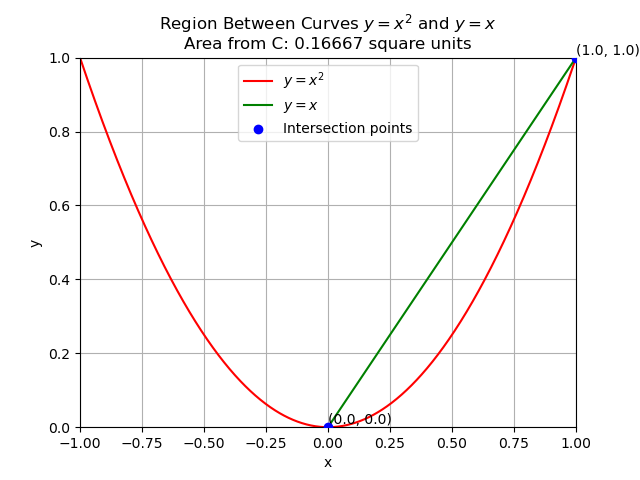
\includegraphics[width=0.5\linewidth]{fig.png}
    \caption{Stem Plot of y\brak{n}}
    \label{fig}
\end{figure}

\end{document}

